\documentclass[]{article}
\usepackage[left=1in,top=1in,right=1in,bottom=1in]{geometry}


%%%% more monte %%%%
% thispagestyle{empty}
% https://stackoverflow.com/questions/2166557/how-to-hide-the-page-number-in-latex-on-first-page-of-a-chapter
\usepackage{color}
\usepackage[table]{xcolor} % are they using color?

\definecolor{WSU.crimson}{HTML}{981e32}
\definecolor{WSU.gray}{HTML}{5e6a71}

\definecolor{shadecolor}{RGB}{248,248,248}
\definecolor{WSU.crimson}{RGB}{152,30,50} % use http://colors.mshaffer.com to convert from 981e32
\definecolor{WSU.gray}{RGB}{94,106,113}

%%%%%%%%%%%%%%%%%%%%%%%%%%%%

\newcommand*{\authorfont}{\fontfamily{phv}\selectfont}
\usepackage{lmodern}


\usepackage[T1]{fontenc}
  \usepackage[utf8]{inputenc}




\usepackage{abstract}
\renewcommand{\abstractname}{}    % clear the title
\renewcommand{\absnamepos}{empty} % originally center

\renewenvironment{abstract}
 {{%
    \setlength{\leftmargin}{0mm}
    \setlength{\rightmargin}{\leftmargin}%
  }%
  \relax}
 {\endlist}

\makeatletter
\def\@maketitle{%
  \pagestyle{empty}
  \newpage
%  \null
%  \vskip 2em%
%  \begin{center}%
  \let \footnote \thanks
    {\fontsize{18}{20}\selectfont\raggedright  \setlength{\parindent}{0pt} \@title \par}%
}
%\fi
\makeatother







\usepackage{graphicx,grffile}
\makeatletter
\def\maxwidth{\ifdim\Gin@nat@width>\linewidth\linewidth\else\Gin@nat@width\fi}
\def\maxheight{\ifdim\Gin@nat@height>\textheight\textheight\else\Gin@nat@height\fi}
\makeatother
% Scale images if necessary, so that they will not overflow the page
% margins by default, and it is still possible to overwrite the defaults
% using explicit options in \includegraphics[width, height, ...]{}
\setkeys{Gin}{width=\maxwidth,height=\maxheight,keepaspectratio}


\title{\textbf{\textcolor{WSU.crimson}{Will V. Denzel}}  }
 

%  

% \author{ \Large true \hfill \normalsize \emph{} }
\author{\Large Joshua
Bennett\vspace{0.05in} \newline\normalsize\emph{Washington State
University}  }


\date{December 14, 2020}
\setcounter{secnumdepth}{3}

\usepackage{titlesec}
% See the link above: KOMA classes are not compatible with titlesec any more. Sorry.
% https://github.com/jbezos/titlesec/issues/11
\titleformat*{\section}{\bfseries}
\titleformat*{\subsection}{\bfseries\itshape}
\titleformat*{\subsubsection}{\itshape}
\titleformat*{\paragraph}{\itshape}
\titleformat*{\subparagraph}{\itshape}

% https://code.usgs.gov/usgs/norock/irvine_k/ip-092225/


%\titleformat*{\section}{\normalsize\bfseries}
%\titleformat*{\subsection}{\normalsize\itshape}
%\titleformat*{\subsubsection}{\normalsize\itshape}
%\titleformat*{\paragraph}{\normalsize\itshape}
%\titleformat*{\subparagraph}{\normalsize\itshape}

% https://tex.stackexchange.com/questions/233866/one-column-multicol-environment#233904
\usepackage{environ}
\NewEnviron{auxmulticols}[1]{%
  \ifnum#1<2\relax% Fewer than 2 columns
    %\vspace{-\baselineskip}% Possible vertical correction
    \BODY
  \else% More than 1 column
    \begin{multicols}{#1}
      \BODY
    \end{multicols}%
  \fi
}





\usepackage{natbib}
\setcitestyle{aysep={}} %% no year, comma just year
% \usepackage[numbers]{natbib}
\bibliographystyle{./../biblio/ormsv080.bst}



\usepackage[strings]{underscore} % protect underscores in most circumstances




\newtheorem{hypothesis}{Hypothesis}
\usepackage{setspace}


%%%%%%%%%%%%%%%%%%%%%%%%%%%%%%%%%%%%%%%%%%%%%%%%%%%%%
%%% MONTE ADDS %%%

\usepackage{fancyhdr} % fancy header 
\usepackage{lastpage} % last page 

\usepackage{multicol}


\usepackage{etoolbox}
\AtBeginEnvironment{quote}{\singlespacing\small}
% https://tex.stackexchange.com/questions/325695/how-to-style-blockquote


\usepackage{soul}			%% allows strike-through
\usepackage{url}			%% fixes underscores in urls
\usepackage{csquotes}		%% allows \textquote in references
\usepackage{rotating}		%% allows table and box rotation
\usepackage{caption}		%% customize caption information
\usepackage{booktabs}		%% enhance table/tabular environment
\usepackage{tabularx}		%% width attributes updates tabular
\usepackage{enumerate}		%% special item environment
\usepackage{enumitem}		%% special item environment

\usepackage{lineno}		%% allows linenumbers for editing using \linenumbers
\usepackage{hanging}


\usepackage{mathtools}  	%% also loads amsmath
\usepackage{bm}		%% bold-math
\usepackage{scalerel}	%% scale one element (make one beta bigger font)

\newcommand{\gFrac}[2]{ \genfrac{}{}{0pt}{1}{{#1}}{#2} }

\newcommand{\betaSH}[3]{  \gFrac{\text{\tiny #1}}{{\text{\tiny #2}}}\hat{\beta}_{\text{#3}}   }
\newcommand{\betaSB}[3]{              ^{\text{#1}} _{\text{#2}} \bm{\beta} _{\text{#3}}                   }  %% bold
\newcommand{\bigEQ}{  \scaleobj{1.5}{{\ }= } }
\newcommand{\bigP}[1]{  \scaleobj{1.5}{#1 } }





\usepackage{endnotes}  % he already does this ...
\renewcommand{\enotesize}{\normalsize}
% https://tex.stackexchange.com/questions/99984/endnotes-do-not-be-superscript-and-add-a-space
\renewcommand\makeenmark{\textsuperscript{[\theenmark]}} % in brackets %
% https://tex.stackexchange.com/questions/31574/how-to-control-the-indent-in-endnotes
\patchcmd{\enoteformat}{1.8em}{0pt}{}{}

\patchcmd{\theendnotes}
  {\makeatletter}
  {\makeatletter\renewcommand\makeenmark{\textbf{[\theenmark]} }}
  {}{}



% https://tex.stackexchange.com/questions/141906/configuring-footnote-position-and-spacing

\addtolength{\footnotesep}{5mm} % change to 1mm

\renewcommand{\thefootnote}{\textbf{\arabic{footnote}}}
\let\footnote=\endnote
%\renewcommand*{\theendnote}{\alph{endnote}}
%\renewcommand{\theendnote}{\textbf{\arabic{endnote}}}


\renewcommand*{\notesname}{ENDNOTES}

\makeatletter
\def\enoteheading{\section*{\notesname
  \@mkboth{\MakeUppercase{\notesname}}{\MakeUppercase{\notesname}}}%
  \mbox{}\par\vskip-2.3\baselineskip\noindent\rule{.5\textwidth}{0.4pt}\par\vskip\baselineskip}
\makeatother


\renewcommand*{\contentsname}{TABLE OF CONTENTS}

\renewcommand*{\refname}{REFERENCES}


%\usepackage{subfigure}
\usepackage{subcaption}

\captionsetup{labelfont=bf}  % Make Table / Figure bold

%%% you could add elements here ... monte says .... %%%
%\usepackage{mypackageForCapitalH}


%%%%%%%%%%%%%%%%%%%%%%%%%%%%%%%%%%%%%%%%%%%%%%%%%%%%%

% set default figure placement to htbp
\makeatletter
\def\fps@figure{htbp}
\makeatother


% move the hyperref stuff down here, after header-includes, to allow for - \usepackage{hyperref}

\makeatletter
\@ifpackageloaded{hyperref}{}{%
\ifxetex
  \PassOptionsToPackage{hyphens}{url}\usepackage[setpagesize=false, % page size defined by xetex
              unicode=false, % unicode breaks when used with xetex
              xetex]{hyperref}
\else
  \PassOptionsToPackage{hyphens}{url}\usepackage[draft,unicode=true]{hyperref}
\fi
}

\@ifpackageloaded{color}{
    \PassOptionsToPackage{usenames,dvipsnames}{color}
}{%
    \usepackage[usenames,dvipsnames]{color}
}
\makeatother
\hypersetup{breaklinks=true,
            bookmarks=true,
            pdfauthor={Joshua Bennett (Washington State University)},
             pdfkeywords = {T-tests, Histogram, ScatterPlot, correlation
tables},  
            pdftitle={Will V. Denzel},
            colorlinks=true,
            citecolor=blue,
            urlcolor=blue,
            linkcolor=magenta,
            pdfborder={0 0 0}}
\urlstyle{same}  % don't use monospace font for urls

% Add an option for endnotes. -----

%
% add tightlist ----------
\providecommand{\tightlist}{%
\setlength{\itemsep}{0pt}\setlength{\parskip}{0pt}}

% add some other packages ----------

% \usepackage{multicol}
% This should regulate where figures float
% See: https://tex.stackexchange.com/questions/2275/keeping-tables-figures-close-to-where-they-are-mentioned
\usepackage[section]{placeins}



\pagestyle{fancy}   
\lhead{\textcolor{WSU.crimson}{\textbf{ Will V. Denzel }}}
\chead{}
\rhead{\textcolor{WSU.gray}{\textbf{  Page\ \thepage\ of\ \protect\pageref{LastPage} }}}
\lfoot{}
\cfoot{}
\rfoot{}


\begin{document}
	
% \pagenumbering{arabic}% resets `page` counter to 1 
%    

% \maketitle

{% \usefont{T1}{pnc}{m}{n}
\setlength{\parindent}{0pt}
\thispagestyle{plain}
{\fontsize{18}{20}\selectfont\raggedright 
\maketitle  % title \par  

}

{
   \vskip 13.5pt\relax \normalsize\fontsize{11}{12} 
   
\textbf{\authorfont Joshua Bennett} \hskip 15pt \emph{\small Washington
State University}   

}

}








\begin{abstract}

    \hbox{\vrule height .2pt width 39.14pc}

    \vskip 8.5pt % \small 

\noindent In this Article we will discuss who is the better artor
between Will Smith and Denzel Washington.


\vskip 8.5pt \noindent \textbf{\underline{Keywords}:} T-tests,
Histogram, ScatterPlot, correlation tables \par

    




    
    \hbox{\vrule height .2pt width 39.14pc}
    \vskip 5pt 
    \hfill \textbf{\textcolor{WSU.gray}{ December 14, 2020 } }
    \vskip 5pt 
    
\end{abstract}


\vskip -8.5pt



 % removetitleabstract

\noindent  

\section{Introduction}
\label{sec:intro}

\section{Methods of finding issues in the Data}

\section{Research Question:  What is my primary question}

My primary question for this is who is objectively a better actor?
\label{sec:rq}

\subsection{What is my secondary question}

My secondary question would be what quantifies what a good actor is?
Movie monetary returns? reviews? \label{sec:rq2}

\subsection{What is my other secondary question}

How did the success change over time? (this might be a good factor for
determining acting skill) \label{sec:rq3}

\section{Data Description}
\label{sec:data}

This is a large IMDB dataset that was harvested by my professor Monte
Shaffer. It was taken from the IMBD website in September of 2020. The
data is following Will Smith and Denzel Washington's careers. The movies
that they have been in and the reviews and gross that the movie
made.There was numerous other categories that the data has as well, such
as the Titles of the movies that they were in the rating of the movie
(R,PG-13, PG) a description of the movie how many votes the movie has
and the year it was released. It was compiled and uploaded by my
professor as well to be able to be access and the data analyze in
Rstudio.

\subsection{Summary of Sample}

This is a summary of the Data Set that was used for this
analysis\footnote{summary of Will and Denzels data}

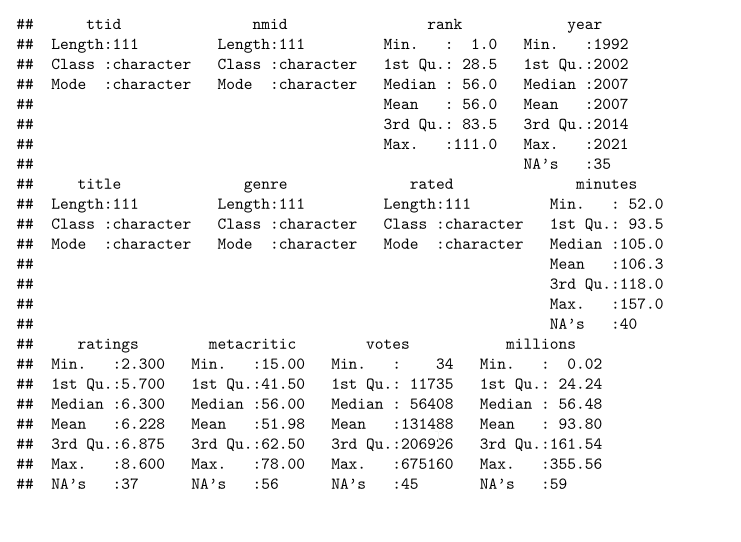
\includegraphics{C:/Users/Galac/Desktop/git419/Stats419_FALL2020/Final/New folder/will PDF summary.png}
summary of Wills data
\footnote{This is an overview of the data I went through to come up with a conclusion.}

\includegraphics{C:/Users/Galac/Desktop/git419/Stats419_FALL2020/Final/New folder/denzel PDF summary.png}
summary of Denzels data
\footnote{This is an overview of the data I went through to come up with a conclusion.}

\label{sec:data-sample}

\subsection{Summary Statistics of Data}

Using the Data given to us by our professor from IMDB, I used the will
dataframe and the Denzel dataframe to work through the data. There were
multiple different methods that I used and they were mostly comparing
the two dataset against each other and other factors of their own. For
example, we took the will dataframe and took the data from the
``metacritic'' column and compared it to the years the movies came out
and you can clear see a downward trend. I would also do the same for the
Denzel dataframe to check for similar results.

I also used multiple T-Tests to judge the data as well as some
Histograms with a Shapiro Normality test. This was to show the mean and
standard deviation between the variable that was being tested. To help
show the trends over time, I implemented a Albine line that intersects
the plot to show the general trajectory of the data. This shows if time
goes by how do their movies change? Was there an initial burst of
popularity that caused the actor to be popular and that wore off? or do
their acting chops shine through giving the ability to keep a steady
straight line. Maybe even improving. Running the welchs T-Test we see a
p-value of 0.001401 which shows that there isn't a statistically
significant difference between them, but if you look at the mean of the
data you see that Will Smiths mean is 6.328 over his career and Denzels
is 6.852 and the standard deviation is .913 to .654. So a strong
indicator of quality. You can also look at the graphs for the
differences between their ``millions'' category (movie earnings). From
Will smith you can clearly see That he has made movies that completely
smash in the box office but still has a trend of only slightly rising.
That might not even account for inflation. But he still averaged over
his career around 50 million more. When comparing their movie gross
there was a 95\% confidence interval of 21.695 to 80.82291.

Correlation tables were also run, but we didn't get much out of it that
we didn't find using other methods.

\label{sec:data-summary}

\section{Key Findings}

After going through this Will v Denzel dataset. We found many
interesting things. Looking at the amount of money over time they make
as well as their reviews over time I found to be the most interesting
ways to look at the data. When comparing reviews against each other from
the start of their careers you can see a much more consistent line for
Denzel Washington and a mean of 6.8 for his movies with will smith
having an average of 6.3 for his movies. While that doesn't appear at
face value to be a significant difference in quality, the biggest thing
to take into account for this is the trend over time. Will Smith has a
significant downward trend whereas Denzel has only a slight downward
trend. This could be due to movie critics being harder on movies
nowadays, but the difference over time is significant in Denzels favor.
The most telling of the findings is when looking at the Denzel movie
gross vs the Will Smith movie gross over time. Will Smiths movie gross
is almost a straight line across the graph from the moment he became a
movie star he has averaged almost the same gross. But for Denzel his
average is in a constant state of going up. Overtime his movies are
getting more and more revenue, whereas Wills is staying almost the same.
Running the correlation tables as well will show a .001 significance.

\label{sec:findings}

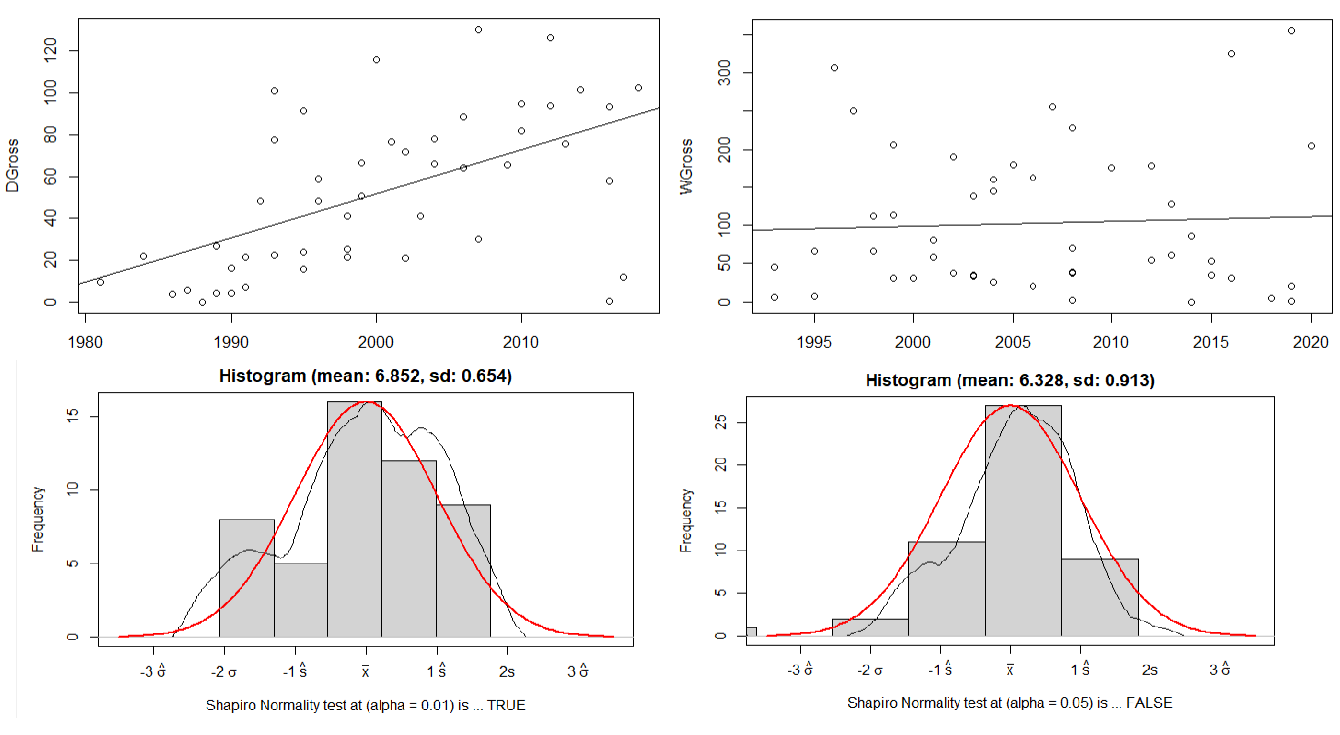
\includegraphics{C:/Users/Galac/Desktop/git419/Stats419_FALL2020/Final/New folder/Combined.png}
Overview of the important data. Will is on the right, Denzel on the left
\footnote{Showing the differences between the two actors in the most importany metrics}

\section{Conclusion}

After going through this Will v Denzel dataset. I can see a clear winner
in my mind, with one graph specifically being my main reason for my
thoughts on the who is the better actor. Starting from the beginning,
will Smith clearly makes more money per movie on average. I wish we had
the data to go through of how much the actors were paid, but without
that we can still make a solid conclusion of who is the better actor.
While Will Smiths movies have made more money they haven't been
consistent at all. This is similar for all the different methods
statistical methods that I used to check. Denzel is consistent and Will
is not. So to choose who the better actor is we need to quantify what
makes an actor good. From the data I gathered, I think Denzel is clearly
the better actor. His movies are constantly going up for how much he is
making, he has significantly more consistent reviews, whereas Will has
some reviews that are down at around 15\%, Denzels lowest is at 30\% and
it was an outlier. Will has 12 movies below a 40\% and Denzel has only
2. The graphic that I found to be the most damning was the Shapiro
Normality test, Wills failed and Denzel you can see just how stable his
gross and reviews are, and how varied Will's is. Denzel is a more
conistent actor which directly plays into acting ability, if he is the
star of the movie and his movies constantly are rated better over 30
years. It has to be the abilities of the actor. There are arguments to
be made the Will is the more successful actor, but not the BETTER actor.
Going by average reviews and income overtime, Denzel Washington is the
better actor. \label{sec:conclusion}

\section{Appendix}
\subsection{Data Provenance}
\subsubsection{Data Collection and organization}

The beginning of the Data Provenance would be the method of collection
collected. For my Data Collection personally, it was collected through
our instructor. He then took that data and combined it into a much
larger Data Set that we could Analyze with much more efficiency. The
functions that are used to manipulate the data are in my RMD file for
this that I used to look at all the data, as well as in the Functions
folder on GitHub. I then organized the data by using the Will and Denzel
dataframes, playing around with the different columns to see what
results we could pull out. Doing this gave me results that I could
compare against each other to judge the actors abilities.




%% appendices go here!


\newpage
\theendnotes

%%%%%%%%%%%%%%%%%%%%%%%%%%%%%%%%%%%  biblio %%%%%%%%
\newpage
\begin{auxmulticols}{2}
\singlespacing 
\bibliography{./../biblio/master.bib}

%%%%%%%%%%%%%%%%%%%%%%%%%%%%%%%%%%%  biblio %%%%%%%%
\end{auxmulticols}

\newpage
{
\hypersetup{linkcolor=black}
\setcounter{tocdepth}{3}
\tableofcontents
}



\end{document}